%======================================================================
\section{Experiments}
\label{sec:exp}
%======================================================================

We validate the framework on automated scholarly review through a diagnose-then-intervene design: Study~1 establishes the pathologies of LLM review panels (Section~\ref{sec:study1}) and their cross-model generality (Section~\ref{sec:crossmodel}); Study~2 applies the framework's three layers as targeted interventions (Sections~\ref{sec:study2a}--\ref{sec:study2c}).

\subsection{Experimental Setup}
\label{sec:setup}

\paragraph{Dataset.}
We assemble 300 papers from the ICLR~2024 conference on OpenReview~\cite{openreview2024iclr}, stratified into three tiers of 100 by official decision and mean reviewer score: \emph{clear-accept} (Oral/Spotlight), \emph{borderline} (poster with mean score nearest to the acceptance boundary), and \emph{clear-reject} (lowest-scoring rejections). Each paper contributes its title, abstract, keywords, official decision, and human reviewer scores. The official decision serves as a noisy ground truth; we therefore treat decision agreement as a \emph{safety} endpoint and behavioral health as the \emph{primary} endpoint (below).

\paragraph{AEIC-Review protocol.}
Each reviewer agent produces a structured review instantiating the AEIC decomposition (Section~\ref{sec:aeic}): Assumption (the paper's claimed contributions), Evidence (a list of $(+)$/$(-)$-tagged strengths and weaknesses anchored to the paper), Inference (overall reasoning), and Conclusion (a stance prefix \texttt{Accept}/\texttt{Weak Accept}/\texttt{Weak Reject}/\texttt{Reject} plus a 1--10 rating). The explicit Conclusion field makes stance and rating extraction reliable across models; reviewer personas differ only in decoding temperature. This field is the measurement basis for every behavioral metric in this paper: stances and ratings are read off structured fields, never inferred from free text.

\paragraph{Conditions.}
Each paper is reviewed by a homogeneous panel of 5 reviewer agents under three conditions: \textbf{parallel} (independent reviews, single round), \textbf{debate} (three rounds; after round~1 each reviewer observes anonymized peer positions and may revise), and \textbf{star} (independent reviews plus a meta-reviewer synthesis). Study~2 adds \textbf{debate-regulated} (Section~\ref{sec:study2b}). Default panels use DeepSeek-V3~\cite{deepseek2024v3}; cross-model panels use GLM-4-Flash~\cite{glm2024chatglm} and DeepSeek-R1~\cite{deepseekai2025r1} on a matched 150-paper subset (first 50 per stratum).

\paragraph{Metrics.}
\emph{Behavioral health} (primary): minority elimination rate and flip direction (an r1 minority reviewer is \emph{eliminated} if their final stance equals the r1 majority; otherwise they \emph{persist}); rating variance collapse ($1 - \bar{\sigma}_{r3}/\bar{\sigma}_{r1}$); mean rating drift. \emph{Decision quality} (safety): agreement of panel decisions with the official outcome, overall and per stratum. \emph{Calibration}: MAE of panel mean rating vs.\ human mean score. Statistics: exact binomial test (flip direction), Wilcoxon signed-rank (paired continuous), McNemar (paired decisions), Wilson 95\% CIs.

\subsection{Study 1: Diagnosis of LLM Review Panels}
\label{sec:study1}

\paragraph{Independent reviews carry a systematic reject bias.}
On clear-accept papers (officially Oral/Spotlight), independent DeepSeek-V3 reviewers accept only 14.4\% of the time; the borderline and clear-reject strata sit at 9.9\% and 4.0\% (Figure~\ref{fig:s1}). The bias is a property of the single-agent prior, not of aggregation---and it is exactly the pathology that Study~2a's calibrated layer targets.

\begin{figure}[t]
\centering
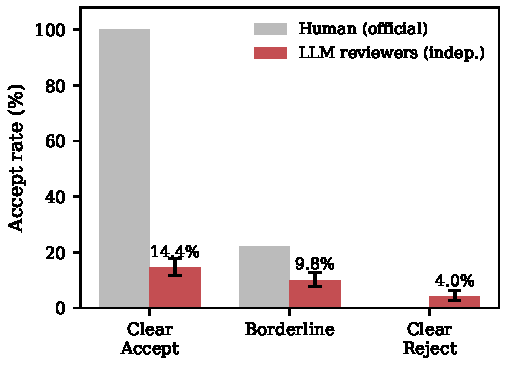
\includegraphics[width=0.49\columnwidth]{figures/fig_s1_negativity_bias.pdf}\hfill
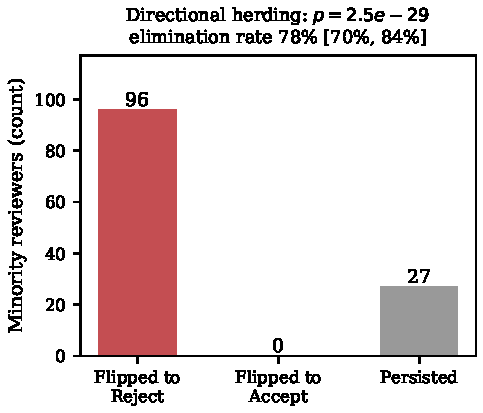
\includegraphics[width=0.49\columnwidth]{figures/fig_s1_minority_fate.pdf}
\caption{Study~1 diagnosis. Left: independent accept rate per stratum vs.\ the official base rate---a systematic reject bias. Right: fate of round-1 minority positions after three discussion rounds: flips run 96:0 toward rejection.}
\label{fig:s1}
\end{figure}

\paragraph{Discussion triggers a negative ratchet.}
Across the 90 panels with a non-unanimous first round, minority positions are eliminated at 78.0\% (Wilson 95\% CI $[69.9, 84.5]$), and flips are entirely one-directional: 96 toward rejection, 0 toward acceptance, 27 persist (binomial $p{=}2.5{\times}10^{-29}$). Panel rating variance collapses by 51.1\% (Wilcoxon $p{=}3.9{\times}10^{-32}$) and mean ratings drift by $-0.25$ points ($p{=}1.0{\times}10^{-32}$). Roughly 70\% of panels are already unanimous after round~1, so discussion predominantly compresses---it rarely deliberates.

\paragraph{Discussion yields no decision benefit.}
Decision agreement with the official outcome is statistically flat across conditions: parallel 61.7\%, debate r1 61.3\%, debate r3 59.7\%, star meta-review 60.7\% (all pairwise McNemar $p{>}0.05$). Three rounds of discussion thus destroy diversity without buying decision quality---the signature pathology that Study~2c's routing layer exploits. Figure~\ref{fig:s1b} summarizes the collapse and the flat decision profile.

\begin{figure}[t]
\centering
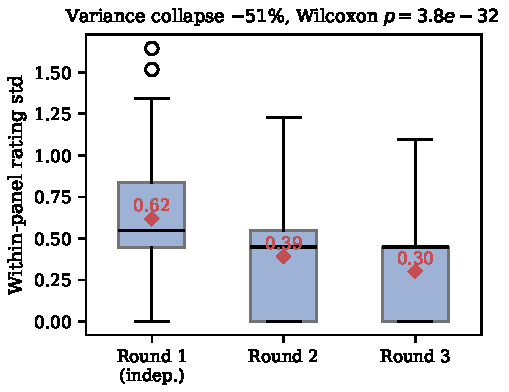
\includegraphics[width=0.49\columnwidth]{figures/fig_s1_variance_collapse.pdf}\hfill
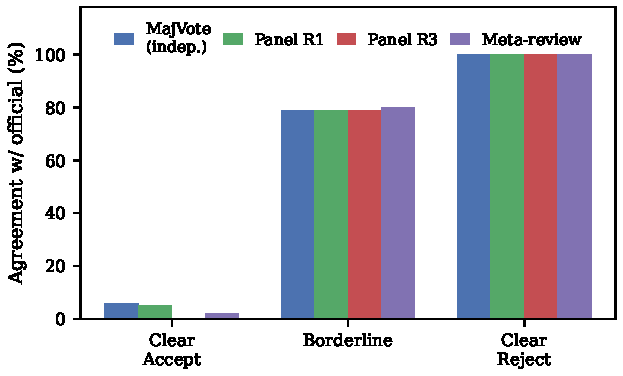
\includegraphics[width=0.49\columnwidth]{figures/fig_s1_decision_accuracy.pdf}
\caption{Left: per-paper rating std, round 1 vs.\ round 3---variance collapses by 51\%. Right: decision agreement by condition---discussion and meta-review add nothing over independent aggregation.}
\label{fig:s1b}
\end{figure}

\subsection{Cross-Model Generality: Opposite Pathological Attractors}
\label{sec:crossmodel}

We replicate the debate condition on a matched 150-paper subset with homogeneous panels of GLM-4-Flash and DeepSeek-R1 (Figure~\ref{fig:s2}). Herding is universal---every model eliminates $\geq$83\% of minorities---but its \emph{direction} is model-dependent. DeepSeek-V3 and R1 panels ratchet toward rejection (100\% and 90\% of flips; accept baserates $\leq$19\%), whereas GLM-4-Flash panels ratchet toward \emph{acceptance} (0\% of flips toward rejection; accept baserate $\geq$97.6\%; 94.4\% of conclusions written as hedged ``Accept/Reject'' forms whose stance must be derived from the rating). Most strikingly, the strongest reasoner does not herd least: R1 achieves the best decision agreement (67.3\%) yet the largest variance collapse (76.4\%), versus 54.0\% for V3 and 12.3\% for GLM (whose panels begin near-unanimous). Capability does not protect against herding; it merely selects the attractor. GLM's near-total conformity also caps its decision quality at 38.7\%, 28.6pp below R1.

\begin{figure}[t]
\centering
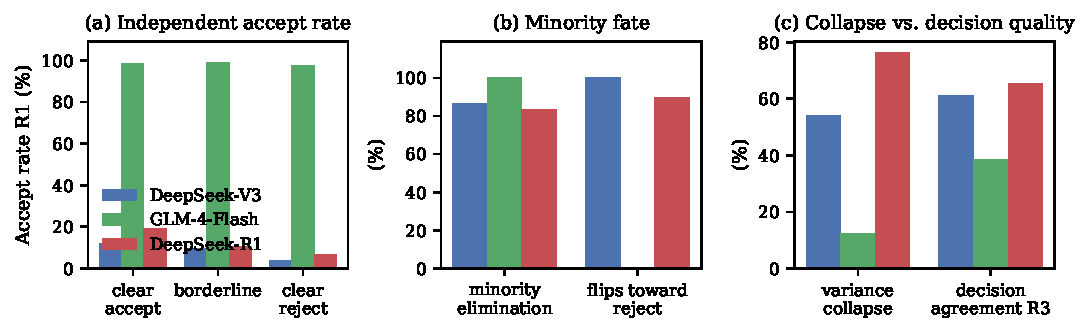
\includegraphics[width=\columnwidth]{figures/fig_s2_crossmodel.pdf}
\caption{Cross-model replication on the matched 150-paper subset. (a)~Independent accept rate per stratum: V3 and R1 are reject-biased, GLM is accept-biased. (b)~Minority elimination is universal ($\geq$83\%), but flip direction is model-dependent. (c)~The strongest reasoner (R1) suffers the largest variance collapse.}
\label{fig:s2}
\end{figure}

\subsection{Study 2a: Calibrated Aggregation Repairs the Reject Bias}
\label{sec:study2a}

The static Stackelberg layer optimizes aggregation parameters $\theta$ on a stratified train split (150 papers): per-reviewer weights $w_i$, signal weights on evidence specificity and $(+)$/$(-)$ balance, a calibration bias $\tau$, and a decision threshold, maximizing agreement minus $\lambda{\times}$calibration MAE (differential evolution; test-only reporting on the held-out 150). Learned $\theta^*$ exhibits a strong positive calibration $\tau{=}+1.04$---the optimizer's direct answer to the diagnosed reject bias---and upweights evidence-specific reviews ($\gamma_1{=}+1.09$).

\begin{table}[t]
\caption{Test-set decision agreement with official outcomes ($n{=}150$). $\theta^*$ repairs the clear-accept stratum from near-zero; most of the gain is already captured by re-thresholding the plain mean (trained threshold). MAE vs.\ human mean score.}
\label{tab:study2a}
\centering\small
\begin{tabular}{@{}lccccc@{}}
\toprule
Method & Overall & Clear-acc. & Borderline & Clear-rej. & MAE \\
\midrule
Majority vote & 60.0\% & 2.0\% & 78.0\% & 100\% & --- \\
Mean threshold & 66.7\% & 44.0\% & 70.0\% & 86.0\% & 1.18 \\
Meta-review (star) & 60.0\% & --- & --- & --- & --- \\
$\theta^*$ aggregation & 64.7\% & 38.0\% & 68.0\% & 88.0\% & 1.14 \\
\bottomrule
\end{tabular}
\end{table}

Table~\ref{tab:study2a} shows the result. Against majority vote, $\theta^*$ lifts clear-accept agreement from 2.0\% to 38.0\% and overall agreement by +4.7pp (McNemar $b{=}20$, $c{=}13$, $p{=}0.30$). A honest baseline check tempers the claim: re-thresholding the plain mean reaches 66.7\% overall. In a \emph{homogeneous} pool, calibration---in any form---is necessary and nearly sufficient; reviewer- and signal-level weighting adds little, consistent with the QA-domain finding that quality signals carry little discriminative power when agents share one backend.

\subsection{Study 2b: Prompt-Level Regulation Cannot Break the Ratchet}
\label{sec:study2b}

The dynamic layer instantiates direction-neutral, evidence-anchored regulation: whenever a panel is non-unanimous, minority reviewers are instructed to change position only if peers rebut specific Evidence items (and to cite the rebutting evidence if they do), while majority reviewers must ground persuasion in specific rebuttals rather than headcounts. On the 89 of 300 panels where the intervention fires (173 minority injections), elimination drops only 78.0\%$\to$71.0\%, variance collapse is unchanged (51.1\%$\to$52.4\%), and intervened minorities persist at 29\% versus 28\% for matched unregulated controls; flips still run 87:1 toward rejection. Decision agreement is preserved (59.7\%$\to$60.7\%)---the safety endpoint holds. On GLM panels the intervention fires rarely (7\% of panels, since round-1 unanimity is near-total) and never rescues a minority (0/7). We report this as a negative result with a clear implication: \emph{rhetorical} anchoring cannot overcome capability-driven conformity; effective regulation must act on the aggregation mechanism or the deliberation structure, not on phrasing.

\subsection{Study 2c: Routing Demotes Discussion to an On-Demand Resource}
\label{sec:study2c}

Since ${\sim}$70\% of panels are unanimous after round~1, deliberation is wasted on most papers. The routing layer selects per paper among four protocols---$\theta^*$ independent aggregation (5 calls), unregulated debate (15), regulated debate (15), meta-review (6)---using round-1-prospective features (stance entropy, rating mean/std, evidence specificity, evidence balance, inference length) with per-action logistic scorers estimating P(correct) on the train split.

\begin{table}[t]
\caption{Test-set routing vs.\ fixed protocols ($n{=}150$). The router matches the best fixed protocol at less than half the deliberation cost; the oracle shows headroom that round-1 features do not unlock.}
\label{tab:study2c}
\centering\small
\begin{tabular}{@{}lcc@{}}
\toprule
Policy & Agreement & Avg.\ calls/paper \\
\midrule
Fixed $\theta^*$ independent & 64.7\% & 5.0 \\
Fixed debate & 58.7\% & 15.0 \\
Fixed debate-regulated & 60.7\% & 15.0 \\
Fixed meta-review & 60.0\% & 6.0 \\
Rule baseline (unanimous$\to$independent) & 60.0\% & 6.0 \\
\midrule
Router (argmax) & 64.7\% & 6.6 \\
Router (cost-sensitive) & 64.7\% & 5.3 \\
Oracle & 74.7\% & 5.3 \\
\bottomrule
\end{tabular}
\end{table}

Table~\ref{tab:study2c} shows that the router ties the best fixed protocol (64.7\%) at 6.6 calls per paper---a 56\% cost reduction versus always discussing (13.4$\times$ fewer calls than the 15-call protocols on 83\% of papers)---and its action mix (124/150 $\theta^*$-independent, 22 regulated-debate, 4 others) directly reflects the Study~1 finding that discussion rarely adds decision value. The 10pp oracle gap indicates headroom that round-1 features cannot yet unlock, a direction for richer prospective signals. Figure~\ref{fig:s3} summarizes all three interventions.

\begin{figure}[t]
\centering
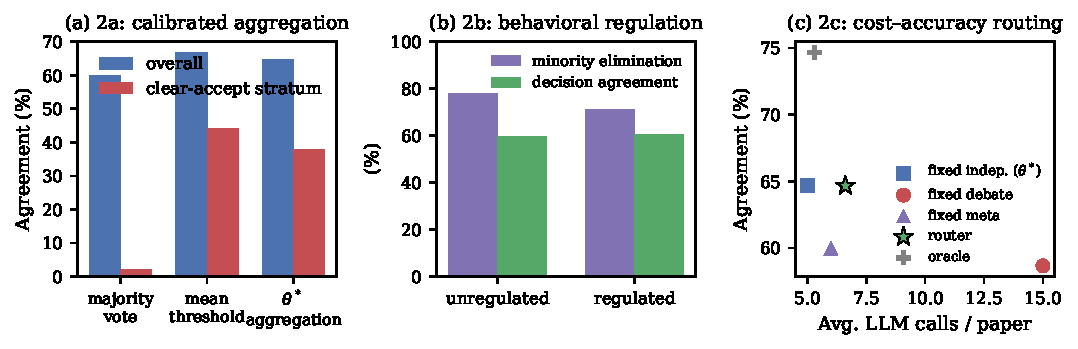
\includegraphics[width=\columnwidth]{figures/fig_s3_interventions.pdf}
\caption{Study~2 interventions. (a)~Calibrated aggregation repairs the clear-accept stratum. (b)~Prompt-level behavioral regulation barely moves minority elimination while preserving decision agreement. (c)~Routing matches the best fixed protocol at the cost frontier.}
\label{fig:s3}
\end{figure}
